\documentclass[letterpaper]{article}
\usepackage[submission]{aaai2027}
\usepackage[hyphens]{url}
\usepackage{graphicx}
\urlstyle{rm}
\def\UrlFont{\rm}
\usepackage{natbib}
\usepackage{caption}
\frenchspacing
\usepackage{booktabs}
\usepackage{amsmath}

\pdfinfo{
/TemplateVersion (2027.1)
}

\setcounter{secnumdepth}{0}

\title{Temporal Referent Integrity in Tool-Using LLM Agents}
\author{Anonymous Submission}
\affiliations{}

\begin{document}
\maketitle

\begin{abstract}
Tool-using language agents operate in environments that may change while a task is being executed. Existing evaluations often ask whether agents update beliefs when observations change. We study a complementary requirement: when should an agent not update the referent of a user's target description? We introduce temporal referent integrity (TRI), the requirement that an agent distinguish references that bind to an entity before an observation update from references that should be evaluated after the update. We construct paired tasks that cross binding time (anchored vs.\ dynamic) with environmental updates. In a state-overwrite controller, which retains the original goal and latest observation but not the previously bound entity, three model families show a sharp contrast: they drift on anchored-flip tasks while remaining largely correct on dynamic-flip controls. GLM-5.1 drifts in 97.0\% of 33 anchored-flip cases and succeeds in 100.0\% of 21 dynamic-flip cases; Qwen3.5 obtains 0.0\% and 100.0\% accuracy over 15 all-paraphrase tasks per condition; MiniMax-M2.5 obtains 0.0\% and 93.3\%. A local stateful tool loop reproduces the same pattern. Automatic compile-then-act controllers repair the core flip failure by persisting binding time and entity identity. A lifecycle stress suite further shows that entity validity is a separate necessary field: full ledgers solve all oracle cases, while automatic compilers still fail on action-specific invalidity. These results suggest that reliable agents need referent lifecycle state, not only updated observations and re-evaluable natural-language goals.
\end{abstract}

\section{Introduction}

Consider two instructions to a tool-using agent:
(i) ``First identify the currently highest-severity incident. After refreshing, escalate that same incident.'' 
(ii) ``Refresh first. Then identify the currently highest-severity incident and escalate it.''
The two instructions use similar words, but they impose different temporal semantics. The first binds an entity before the refresh. The second intentionally evaluates the referring expression after the refresh. If a refresh changes which incident has the highest severity, a reliable agent must preserve the first target but update the second.

This distinction is easy to lose in LLM-agent controllers. Many controllers carry a natural-language goal forward while updating the environment state. If the controller later sees only the latest state and the original goal, a phrase such as ``the currently highest-severity incident'' can be re-evaluated against the wrong state. The agent may confidently act on the new incident, even though the user had already bound the old one.

We call this failure referent drift and study the broader property of temporal referent integrity. TRI is not simply memory retention, dynamic-environment adaptation, or referential ambiguity. The central question is not whether the world changed, but whether a referring expression should be re-bound after the world changes.

\begin{figure*}[t]
\centering
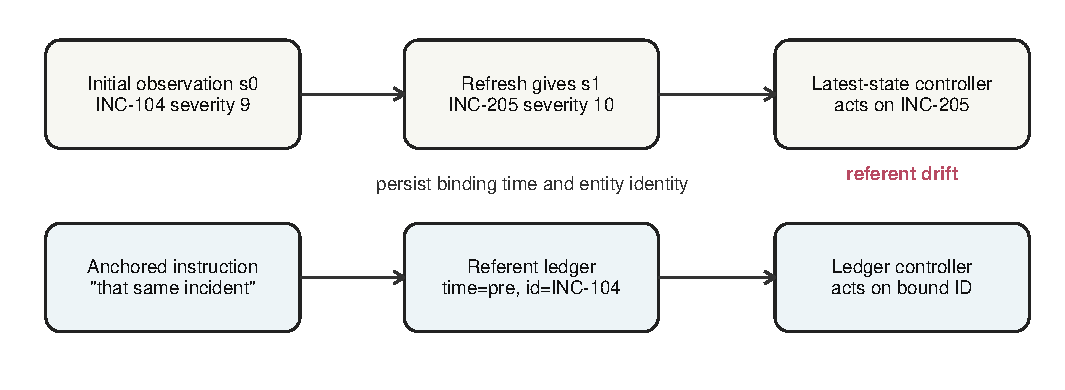
\includegraphics[width=0.92\textwidth]{figures/tri_mechanism_flow.pdf}
\caption{Mechanism of referent drift. A latest-state controller re-evaluates an anchored selector after refresh, while a referent ledger preserves binding time and entity identity.}
\label{fig:mechanism}
\end{figure*}

This paper makes four contributions. First, we define temporal referent integrity as a sufficient-state requirement for tool-using agents. Second, we introduce paired and lifecycle benchmarks that isolate binding time, entity identity, selector re-evaluation, and validity. Third, we show that state-overwrite and lossy-summary controllers produce mechanism-specific referent drift across models and paraphrases, including in a stateful tool loop. Fourth, we propose a typed temporal reference ledger and an automatic compile-then-act controller that repairs the core flip failure while exposing action-specific validity as a remaining challenge.

\section{Temporal Referent Integrity}

Let $s_0$ be the initial observation, $s_1$ a later observation after a refresh, and $r$ a referring expression in the user's instruction. An anchored reference binds before the update:
\[
    target = bind(r, s_0).
\]
A dynamic reference binds after the update:
\[
    target = bind(r, s_1).
\]
Temporal referent integrity requires the agent to preserve this binding-time distinction even when $bind(r,s_0) \ne bind(r,s_1)$.

\begin{table}[t]
\centering
\small
\begin{tabular}{lll}
\toprule
Binding & Update & Correct Behavior \\
\midrule
Anchored & Flip & preserve pre-refresh entity \\
Anchored & Stable & preserve same entity \\
Dynamic & Flip & select post-refresh entity \\
Dynamic & Stable & select same entity \\
\bottomrule
\end{tabular}
\caption{Core TRI design. The anchored-flip condition is the critical counterexample.}
\label{tab:design}
\end{table}

TRI is also a sufficient-state problem. A controller state containing only the latest observation and the original natural-language goal is not sufficient for anchored references. A sufficient referent state should include
\[
z = (r, \tau_b, e, q, v, p),
\]
where $r$ is the referring expression, $\tau_b$ is binding time, $e$ is the bound entity identity, $q$ is the selector for dynamic evaluation, $v$ is the validity condition for acting on a bound entity, and $p$ is provenance for the observation that licensed the binding. This framing turns the failure from a generic forgetting error into a representation claim: latest-state summaries can be insufficient even when the latest observation is accurate.

\textbf{Why latest state is insufficient.} Suppose two tasks share the same natural-language goal suffix, the same refreshed state $s_1$, and the same surface referring expression $r$, but differ in binding time. In the anchored task, the correct target is $bind(r,s_0)$; in the dynamic task, it is $bind(r,s_1)$. If an update flips the selector so that $bind(r,s_0)\ne bind(r,s_1)$, then any deterministic controller whose action state is restricted to $(r,s_1)$ must return the same target for both tasks. It therefore cannot be correct on both. The missing variable is not a more accurate latest observation, but the temporal binding record that distinguishes whether $r$ has already been resolved.

\section{Benchmark}

We generate deterministic tasks over structured mini-domains. Each task contains a user instruction, an initial state with stable entity IDs, a refreshed state, an oracle target ID, and a fixed action schema. Domains include incidents, meetings, support tickets, repository branches, shipments, experiment runs, invoices, devices, patient cases, and datasets. Selectors cover numeric maxima, queue position, Boolean selection, default branch, active run, urgent case, and assignment status.

We use five paraphrase families for each anchored/dynamic pair. Some paraphrases are natural, while one explicitly says to bind identity before refresh. Updates include selector-flipping, stable, and removed-entity cases. Scoring is exact string matching over entity IDs; no LLM judge is used.

We also generate a 30-case lifecycle stress suite: five scenarios times three paraphrases times two binding modes. The scenarios test branch rename with selector flip, action-specific invalidity, display-name collision, multiple refreshes before action, and delayed binding. This suite is not used to tune prompts; it checks whether the proposed state fields generalize beyond the original flip/stable/removed grid.

\section{Controllers}

\textbf{Direct and full-history controllers.} These modes test whether the base model can understand the temporal semantics when the relevant history is available.

\textbf{State overwrite.} After refresh, the controller retains only the original instruction and refreshed state. A single-call version gives exactly this representation to the model. This mode simulates agents whose working state is updated to the latest observation without persisting bound entity identities.

\textbf{Memory summaries.} We compare free-form natural memory, compressed memory that forbids entity IDs, and a lossy summary controller in which a model-generated bounded summary is the only state passed to the next step.

\textbf{Temporal reference ledger.} A typed ledger stores binding time, selector, bound target ID, validity condition, and provenance. We test both oracle ledgers and automatic compile-then-act controllers. The compiler first emits a ledger from the instruction and initial observation; the actor then acts from the ledger and refreshed state.

\textbf{Stateful tool loop.} We instantiate each task as an environment with three tools: observe, refresh, and process. Each episode produces an observe-refresh-process trace. We evaluate latest-state, full-history, lossy-summary, and compile-then-act policies in this tool loop.

\section{Method: Temporal Reference Compiler}

The compiler transforms user goals into structured referent records. It performs binding-time inference, selector grounding, identity persistence, and validity checking. The method is intentionally simple: the contribution is not that storing an ID is difficult, but that binding time and validity identify when an ID must be stored, when it must not be used, and when a selector should remain dynamic.

\begin{center}
\centering
\small
\begin{tabular}{@{}p{0.94\columnwidth}@{}}
\toprule
\textbf{Algorithm 1: Compile-then-act for TRI} \\
\midrule
Input: instruction $g$, initial observation $s_0$, refreshed observation $s_1$ \\
1. Extract referring expression $r$ and infer binding time $\tau_b$. \\
2. Ground selector $q$ from $r$ and record provenance $p=s_0$. \\
3. If $\tau_b=pre$, bind $e=bind(q,s_0)$; otherwise leave $e$ unset. \\
4. Compile an action validity predicate $v$ for the intended operation. \\
5. At action time, if $\tau_b=post$, act on $bind(q,s_1)$. \\
6. If $\tau_b=pre$ and $v(e,s_1)$ holds, act on $e$; otherwise return invalid. \\
\bottomrule
\end{tabular}
\end{center}

Formally, action selection is
\[
\begin{cases}
act(e), & \tau_b = pre \land valid(e,s_1) \\
invalid, & \tau_b = pre \land \neg valid(e,s_1) \\
act(bind(q,s_1)), & \tau_b = post.
\end{cases}
\]
In experiments, the oracle ledger uses known task fields, while the automatic compiler asks the model to emit JSON fields for binding time, selector, bound ID, and validity before the actor chooses the final target.

\section{Experimental Setup}

All tasks are deterministic and require no training. API-backed model runs use temperature 0.0 and JSON-only prompts. Outputs are parsed into target IDs with a deterministic parser; malformed or API-failed responses are excluded only in tables that explicitly report valid completed runs. Accuracy is exact match against the oracle target identifier. Drift is counted when an anchored case selects the post-refresh selector winner while the correct answer is the pre-refresh bound entity. We report counts whenever a run is a pilot or a subset, and we do not use an LLM judge. Each JSONL run log stores the task, model name, controller mode, raw model outputs, parsed target, correctness, drift flag, and latency, making the aggregate tables reproducible from saved transcripts.

\section{Results}

\subsection{State Overwrite Causes Paired Referent Drift}

\begin{table}[t]
\centering
\small
\begin{tabular}{llrr}
\toprule
Model & Condition & Acc. & Drift \\
\midrule
GLM-5.1 & anchored (n=33) & 3.0 & 97.0 \\
GLM-5.1 & dynamic (n=21) & 100.0 & 0.0 \\
Qwen3.5 & anchored (n=15) & 0.0 & 73.3 \\
Qwen3.5 & dynamic (n=15) & 100.0 & 0.0 \\
MiniMax & anchored (n=15) & 0.0 & 100.0 \\
MiniMax & dynamic (n=15) & 93.3 & 0.0 \\
DeepSeek & anchored (n=3) & 0.0 & 100.0 \\
DeepSeek & dynamic (n=3) & 100.0 & 0.0 \\
\bottomrule
\end{tabular}
\caption{State-overwrite controllers drift on anchored-flip tasks but succeed on dynamic-flip controls. Values are percentages.}
\label{tab:main}
\end{table}

Table~\ref{tab:main} shows the main mechanism result. The same controller can use the refreshed state correctly when the instruction is dynamic, but it incorrectly re-binds anchored descriptions after refresh. For GLM-5.1, anchored-flip accuracy is 0.0\% for four paraphrase families and 20.0\% for the highly explicit binding paraphrase; explicit wording helps slightly but does not solve the state-representation problem. On held-out domains, GLM-5.1 under state overwrite fails on 20/20 anchored-flip tasks, while valid dynamic held-out responses are correct in 6/6 cases.

\subsection{Stateful Tool Controller Replication}

\begin{table}[t]
\centering
\small
\begin{tabular}{llrr}
\toprule
Controller & Condition & Acc. & Drift \\
\midrule
latest-state & anchored (n=14) & 21.4 & 64.3 \\
latest-state & dynamic (n=15) & 100.0 & 0.0 \\
full-history & anchored (n=3) & 100.0 & 0.0 \\
full-history & dynamic (n=3) & 100.0 & 0.0 \\
lossy-summary & anchored (n=3) & 66.7 & 33.3 \\
lossy-summary & dynamic (n=3) & 100.0 & 0.0 \\
compile-then-act & anchored (n=3) & 100.0 & 0.0 \\
compile-then-act & dynamic (n=3) & 100.0 & 0.0 \\
\bottomrule
\end{tabular}
\caption{GLM-5.1 in a stateful observe-refresh-process tool loop. Latest-state control remains unreliable on all-paraphrase anchored references but succeeds on dynamic controls; full history and compile-then-act repair the p0 failure.}
\label{tab:tool}
\end{table}

Table~\ref{tab:tool} reduces the risk that TRI is only an artifact of hand-constructed prompts. In a stateful tool loop, the latest-state controller processes the wrong post-refresh target on all p0 anchored-flip tasks, and the all-paraphrase expansion remains unreliable. Full-history and compile-then-act controllers repair the p0 failure, and lossy summary partially fails. This is a local tool environment rather than ToolSandbox or AppWorld \cite{lu2024toolsandbox,trivedi2024appworld}, but it demonstrates that the failure persists in an actual tool-call trajectory.

\subsection{Compiler and Memory Repairs}

\begin{table}[t]
\centering
\small
\begin{tabular}{llrr}
\toprule
Model & Controller & Anchored & Dynamic \\
\midrule
GLM-5.1 & compile & 15/15 & 15/15 \\
Qwen3.5 & compile & 9/9 & 6/6 \\
MiniMax & compile & 6/6 & 6/6 \\
GLM-5.1 & natural memory & 3/3 & -- \\
GLM-5.1 & compressed & 0/3 & 3/3 \\
GLM-5.1 & ledger-safe & 3/3 & -- \\
\bottomrule
\end{tabular}
\caption{Repair and memory results. Compile-then-act uses an automatically generated ledger rather than an oracle ledger.}
\label{tab:repair}
\end{table}

Table~\ref{tab:repair} shows that preserving the right state repairs the failure. For GLM-5.1, binding-time compilation, anchored bound-ID compilation, and final action accuracy are all 100.0\% over 15 anchored-flip and 15 dynamic-flip development tasks. Qwen3.5 and MiniMax-M2.5 compiler pilots also compile binding time correctly and act correctly on all completed tasks.

The memory baselines clarify the mechanism. A free-form natural note can preserve enough identity information in simple tasks, but a compressed note that drops entity IDs and exact values collapses back to state-overwrite behavior. In a lossy summary case study over 15 anchored-flip tasks, 100.0\% of summaries contain temporal anchor words such as ``initial,'' ``original,'' or ``before,'' but 0.0\% contain an entity ID; accuracy falls to 26.7\%. Temporal wording alone is therefore not sufficient controller state.

\subsection{Field Ablation}

\begin{table}[t]
\centering
\small
\begin{tabular}{lrrr}
\toprule
Representation & Anchored & Removed & Dynamic \\
\midrule
raw goal + latest state & 0.0 & 0.0 & 100.0 \\
selector memory & 0.0 & 0.0 & 100.0 \\
binding-time only & 0.0 & 0.0 & 100.0 \\
entity only & 100.0 & 0.0 & 0.0 \\
time + entity & 100.0 & 0.0 & 100.0 \\
full ledger & 100.0 & 100.0 & 100.0 \\
\bottomrule
\end{tabular}
\caption{Oracle representation ablation over all 300 tasks. Entity identity fixes anchored flips but not removed entities; validity is needed for safe behavior.}
\label{tab:ablation}
\end{table}

Table~\ref{tab:ablation} shows that the ledger is not merely ``save an ID.'' Entity identity fixes anchored flips, but fails when the entity is removed. Binding time plus entity fixes dynamic-vs.-anchored selection, but still fails validity. The full ledger handles referent preservation and entity invalidation.

\begin{figure}[t]
\centering
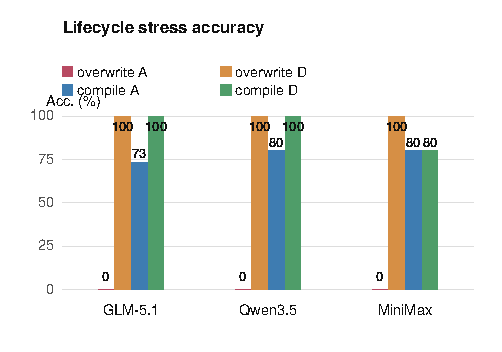
\includegraphics[width=\columnwidth]{figures/lifecycle_accuracy_column.pdf}
\caption{Lifecycle stress-test accuracy from real model runs. GLM-5.1 is evaluated on all 30 lifecycle cases; Qwen3.5 and MiniMax-M2.5 are evaluated on the p0 subset.}
\label{fig:lifecycle}
\end{figure}

\subsection{Lifecycle Stress Test}

\begin{table}[t]
\centering
\small
\begin{tabular}{lrr}
\toprule
Representation & Anchored & Dynamic \\
\midrule
latest-state selector & 0.0 & 100.0 \\
bound name only & 20.0 & 60.0 \\
bound ID only & 80.0 & 0.0 \\
binding-time only & 0.0 & 100.0 \\
time + ID & 80.0 & 100.0 \\
full lifecycle ledger & 100.0 & 100.0 \\
\bottomrule
\end{tabular}
\caption{Oracle representation ablation on 30 lifecycle stress tasks. Values are accuracies over 15 anchored and 15 dynamic cases.}
\label{tab:lifecycle}
\end{table}

Table~\ref{tab:lifecycle} tests whether the ledger fields remain necessary beyond simple selector flips. Latest-state selection again solves dynamic references but fails every anchored case. Name-only memory is brittle under rename and collision. ID-only memory preserves anchored entities when they remain valid, but fails dynamic references and action-invalid cases. Time plus ID solves dynamic-vs.-anchored selection, yet still fails the action-invalid scenario because the bound entity remains present but is no longer actionable. The full lifecycle ledger, which includes validity, is correct on all 30 oracle cases.

We also ran GLM-5.1 on the lifecycle suite. The state-overwrite controller obtains 0/15 anchored accuracy and 15/15 dynamic accuracy. Compile-then-act improves to 11/15 anchored and 15/15 dynamic, solving rename, multi-refresh, delayed binding, and most collision cases. Its remaining failures are informative: all three action-invalid cases process the pre-refresh ID instead of returning invalid, and one explicit collision paraphrase returns invalid for a still-valid bound invoice. Thus automatic compilation substantially mitigates drift, but robust validity compilation remains open.

\section{Related Work}

Stateful tool-use benchmarks such as ToolSandbox and app-like benchmarks such as AppWorld evaluate tool use over changing state and insufficient information \cite{lu2024toolsandbox,trivedi2024appworld}. Dynamic-environment benchmarks such as ClawArena and EvoArena evaluate robustness under evolving information environments \cite{ji2026clawarena,xu2026evoarena}. TRI differs because both adapting and refusing to adapt can be correct depending on binding time.

ReAct-style agents interleave reasoning and acting \cite{yao2022react}; memory-augmented agents store summaries, entities, and retrieved traces \cite{zhang2024memorysurvey,bousetouane2026memorycontrol}. TRI identifies a specific missing variable in such controller state: whether a referring expression has already bound, and to which entity. Work on referential ambiguity asks whether a model can resolve or clarify ambiguous references. TRI can fail even when the initial reference is unambiguous, because the controller later reinterprets it against a new state.

\section{Limitations}

The all-paraphrase paired development matrix is complete for GLM-5.1, Qwen3.5, and MiniMax-M2.5, but DeepSeek-V4-Pro remains a small pilot because the endpoint was unstable in longer runs. The local stateful tool loop strengthens the evidence beyond static prompts, but external ToolSandbox/AppWorld-style replication remains future work. Natural-language memory is a strong baseline on simple tasks; compressed-memory and lossy-summary results are first stress tests. The lifecycle suite covers rename, collision, repeated refresh, delayed binding, and action-specific invalidity, but it is still small. In particular, automatic compile-then-act fails action-invalid cases in the current implementation, showing that validity should be treated as a first-class state and policy problem rather than as a solved post-processing detail.

\section{Conclusion}

Temporal referent integrity exposes a gap in tool-using LLM agents. Agents must not only update their beliefs when the world changes; they must also know which parts of the user's goal should remain fixed. A state-overwrite controller can systematically drift from a pre-refresh entity to a post-refresh entity while handling dynamic references correctly. Typed temporal reference ledgers provide a simple sufficient-state target, and compile-then-act controllers substantially reduce drift. The lifecycle results show why the target representation must include not only binding time and identity, but also validity conditions for action.

\bibliography{tri_references}

\end{document}
